\documentclass{article}
\usepackage[preprint]{neurips_2026}

\usepackage[utf8]{inputenc}
\usepackage[T1]{fontenc}
\usepackage{hyperref}
\usepackage{url}
\usepackage{booktabs}
\usepackage{amsfonts}
\usepackage{amsmath}
\usepackage{microtype}
\usepackage{xcolor}
\usepackage{graphicx}

% This is an ES 678 course paper, not a conference submission.
\makeatletter
\renewcommand{\@noticestring}{ES 678 Course Project}
\makeatother

\title{LegibleRx: Predicting Low-Vision Legibility of Medicine-Pack Text from Images}

\author{%
  Kudumula Vinod Kumar Reddy\\
  Roll Number: 23110178 \\
  ES 678 \\
  Indian Institute of Technology Gandhinagar
}

\begin{document}
\maketitle

\begin{abstract}
People with low vision often cannot read the drug name, strength or expiry date on Indian blister strips. We ask whether
image measurements of a printed text region predict how much simulated vision loss that region survives. The target is an
\emph{OCR-survival} score: the number of steps on an 8-step low-vision ladder (blur, contrast loss, veiling glare) at which
Tesseract still reads the region with character error rate below 10\%. On 1{,}800 regions from 100 \emph{synthetic}
medicine packs photographed under three lightings, with a product-grouped test split, LightGBM on seven hand-measured
feature groups reaches macro-F1 0.81 (95\% CI 0.75--0.86) against 0.59 for a print-guideline rule, a gain of 0.21
(0.14--0.28). Text size, stroke weight and contrast carry most of the signal. All results are on synthetic data and an
OCR proxy; they are not evidence about human readers.
\end{abstract}

\section{Problem and Motivation}
In moderate simulated visual impairment only about 20\% of people could read enough of a typical pharmacy label to take a
medicine correctly \citep{latham2011}. Indian strips add reflective foil, tiny batch/expiry print and crowded layouts.
\textbf{Question:} given a pack photo and a box around one text region, can we predict that region's low-vision legibility
before anyone tries to read it? \textbf{Row:} one text region on one photo. \textbf{Target:} survival score
$y\in\{0,\dots,8\}$ (defined in Sec.~\ref{sec:data}), binned into illegible ($y<3$), borderline ($3\le y<6$) and legible
($y\ge6$). \textbf{Prediction time:} only the clean image crop, its box and its region type (drug name, strength, dosage,
expiry/batch, warning, other) are available; OCR output and degraded images are not used as inputs. \textbf{Claim limit:}
we predict an OCR proxy on synthetic packs; human validation (planned) is not reported here.

\section{Data and Preparation}\label{sec:data}
\textbf{Source.} Real photos were not ready, so we used the fallback in our proposal: a seeded generator renders 100 packs
(foil, white or coloured card; random curvature) with six text fields each, at field-typical font sizes, colours and
weights, and photographs each pack under indoor, daylight and single-bulb glare lighting (camera blur, noise, JPEG). This
gives 300 images and 1{,}800 regions. All data regenerate from the code; nothing private is involved.
\textbf{Quality checks.} No missing values, duplicate ids, degenerate boxes, empty reference text or missing files. An early
version let long names run off the pack, giving large clear text a score of 0; we found this in the error gallery and fixed it.
\textbf{Label.} Images are resized to height 1000\,px so that blur is in pack-relative units. At ladder level
$s\in\{1..8\}$ the crop is blurred with $\sigma=0.45s$, contrast is scaled by $(1-0.08s)$ about the mean and a veil
$g=0.04s$ is added. With $c_s$ the CER at level $s$, $y=0$ if $c_0\ge\tau$, otherwise $y=\max\{k: c_s<\tau\ \forall s\le k\}$, with $\tau=0.10$.
Classes: 669 illegible, 727 borderline, 404 legible.
\textbf{Features} (clean crop only): median connected-component height (x-height), WCAG contrast ratio between ink and
background luminance, specular-glare fraction, baseline curvature, relative stroke width, background edge density, box
geometry and region type. These are fixed measurements with no fitted parameters; the only learned transform (feature
standardisation for the CNN) is fit on the training split.

\section{Methods}
\textbf{Dummy:} dev mean / majority class. \textbf{Rule baseline:} counts violations of x-height $<14$\,px per 1000\,px
($\approx$1.4\,mm on a 10\,cm pack), contrast $<4.5{:}1$ (WCAG) and glare $>5\%$; 0/1/$\ge$2 violations map to
legible/borderline/illegible, and the score prediction is the dev median for that count. It shows what guidelines alone catch.
\textbf{LightGBM} \citep{ke2017}\textbf{:} gradient-boosted trees minimising squared error $\sum_i (y_i-f(\mathbf{x}_i))^2$ on the features; suited to
small tabular data with non-linear thresholds, and explainable with SHAP \citep{lundberg2017}. Classes come from cut-offs
$(c_1,c_2)$ on $\hat y$. \textbf{CNN:} MobileNetV3-Small \citep{howard2019} on the $64\times256$ crop, concatenated with an
MLP on the features, trained with smooth-L1 loss. ImageNet weights could not be downloaded in our run environment, so it
was trained from random initialisation.

\section{Evaluation Design}
Packs, not photos, are the unit of independence: the three photos of a pack share its design. We hold out 20\% of products
(20 products, 360 regions) as the test set; no product appears in both. On the remaining 80 products (dev), LightGBM
hyper-parameters (24-point grid) were chosen by 5-fold GroupKFold MAE, and $(c_1,c_2)$ by maximising macro-F1 on the
out-of-fold predictions, giving $(2.25, 5.25)$. The CNN used a further product-disjoint validation set (12 products) for
early stopping and its cut-offs. Each model was scored once on test. \textbf{Metrics:} MAE and Spearman $\rho$ for the
ordinal score (ranking matters for triage); macro-F1 because classes are unbalanced and every class matters;
quadratic-weighted $\kappa$ because confusing illegible with legible is worse than an adjacent error; illegible recall
because a missed illegible region is the safety-relevant failure. 95\% CIs use a bootstrap that resamples \emph{products}
(1{,}000 draws); $\Delta$F1 vs the rule is paired within each draw.

\section{Results and Error Analysis}
\begin{table}[h]
\centering\small
\caption{Test set (20 held-out products, 360 regions). Brackets: 95\% product-clustered bootstrap CI.}
\label{tab:main}
\begin{tabular}{lcccccc}
\toprule
Model & MAE & Spearman $\rho$ & macro-F1 & $\Delta$F1 vs rule & QWK & Illeg.\ recall\\
\midrule
Dummy & 2.11 & -- & 0.19 & $-0.40$ & 0.00 & 0.00\\
Rule baseline & 1.63 & 0.64 & 0.59 [0.53, 0.66] & -- & 0.60 & \textbf{0.86}\\
LightGBM & \textbf{0.81} & \textbf{0.85} & \textbf{0.81} [0.75, 0.86] & \textbf{+0.21} [0.14, 0.28] & \textbf{0.77} & 0.70\\
CNN (no pretraining) & 1.63 & 0.68 & 0.69 [0.62, 0.75] & +0.10 [0.03, 0.16] & 0.64 & 0.58\\
\bottomrule
\end{tabular}
\end{table}
LightGBM beats the rule baseline by 21 F1 points, above our 10-point target, and the interval excludes zero (Table~\ref{tab:main}).
On safety-critical fields (drug name, strength, expiry) the gap holds (macro-F1 0.77 vs 0.57). The CNN without pretraining
is weaker than the feature model at this data size. \textbf{Important trade-off:} the rule flags more truly illegible
regions (recall 0.86 vs 0.70); its rule is conservative and over-flags, which costs precision. A deployment that cares most
about missed illegible text should lower $c_1$ or combine both. \textbf{Errors.} Error is largest for strength (MAE 1.47)
and drug-name regions (1.10), where only 30\% and 17\% are illegible, and illegible recall there is 0.33 and 0.20: large
text that fails because of glare or poor colour contrast is predicted legible from its size. Small expiry/batch text is easy
(MAE 0.34). Errors are similar across lighting (MAE 0.77--0.88).

\section{Graduate Depth Analysis}
\begin{figure}[h]
\centering
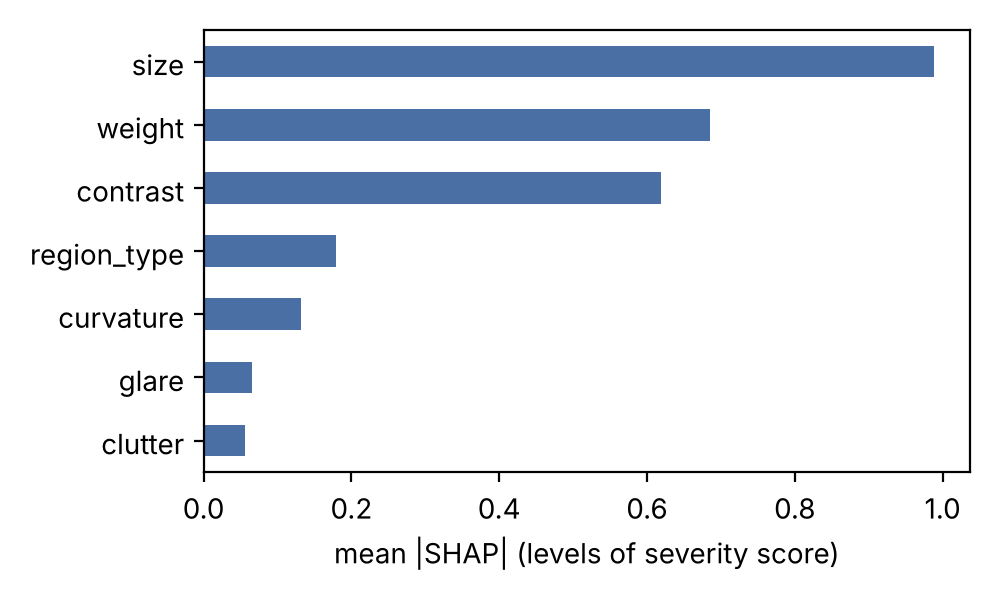
\includegraphics[width=0.42\linewidth]{shap_groups.png}
\caption{Mean $|$SHAP$|$ per feature group (test set, LightGBM).}
\label{fig:shap}
\end{figure}
\textbf{What drives legibility (SHAP and ablation).} Size dominates (mean $|$SHAP$|$ 0.99 levels), followed by stroke
weight (0.69) and contrast (0.62); glare and clutter matter little (Fig.~\ref{fig:shap}). Ablation by GroupKFold on dev
(test untouched) agrees: removing contrast raises CV MAE most (+0.06), then size, weight and region type (+0.03 each);
removing glare or clutter changes nothing. Glare's small role is partly a design artefact: our ladder adds a uniform veil,
not localised specular highlights, so the label itself under-represents foil glare.
\textbf{Is the proxy label stable?} Changing $\tau$ to 0.05 or 0.20 keeps labels highly rank-correlated with $\tau=0.10$
($\rho=0.96, 0.97$) and moves the illegible share from 43\% to 33\%; test macro-F1 stays within 0.75--0.77. Conclusions do
not hinge on the exact CER threshold.
\textbf{Uncertainty.} Split-conformal 90\% intervals \citep{lei2018} calibrated on dev out-of-fold residuals have half-width
1.8 levels and 86\% test coverage, a little under nominal. Coverage is 0.86--0.87 in every lighting but only 0.62 for strength
and 0.75 for drug names, the same subgroups as above: the model is overconfident exactly on large text that fails for
non-size reasons. Group-conditional calibration would be needed before showing intervals to users.
\textbf{Explanations and cost.} For regions predicted not legible, the most negative SHAP group names the fix: size (148),
contrast (73), weight (44). Feature extraction plus prediction take 17\,ms per image (CPU).

\section{Limitations and Conclusion}
The main limitation is validity: the data are synthetic and the label is Tesseract's survival on a simple simulator, not a
human reading test. A stronger claim needs real pack photos and the planned human calibration set (target Spearman
$\rho\ge0.6$ with ratings). Region boxes and types are given, so detection errors are not evaluated, and SHAP shows
association in the model, not causes of illegibility. Within those limits, measured size, stroke weight and contrast
predict the OCR-survival proxy well beyond printing guidelines, but the model misses illegible large text, so it should
complement, not replace, a conservative rule.

\section{Reproducibility and AI-Use Disclosure}
Code, executed notebook, results and this paper: \url{https://github.com/owner/repository} (\texttt{LegibleRx\_colab.ipynb};
seed 42; test products listed in \texttt{results/test\_products.csv}). Synthetic data regenerate from the notebook; no private
data or keys are stored. \textbf{AI use:} Claude (Anthropic) drafted the pipeline code and a first draft of this paper from
our proposal and ran the notebook; we checked the split, metrics and numbers against the result files. \emph{[Edit to match
what you did.]}

\begin{thebibliography}{9}
\small
\bibitem[Latham et al.(2011)]{latham2011} K.~Latham et al. Legibility of pharmacy labels by people with simulated visual impairment. 2011.
\bibitem[Lundberg and Lee(2017)]{lundberg2017} S.~Lundberg and S.-I.~Lee. A unified approach to interpreting model predictions. \emph{NeurIPS}, 2017.
\bibitem[Howard et al.(2019)]{howard2019} A.~Howard et al. Searching for MobileNetV3. \emph{ICCV}, 2019.
\bibitem[Lei et al.(2018)]{lei2018} J.~Lei et al. Distribution-free predictive inference for regression. \emph{JASA}, 2018.
\bibitem[Ke et al.(2017)]{ke2017} G.~Ke et al. LightGBM: a highly efficient gradient boosting decision tree. \emph{NeurIPS}, 2017.
\end{thebibliography}

\end{document}
